% Options for packages loaded elsewhere
% Options for packages loaded elsewhere
\PassOptionsToPackage{unicode}{hyperref}
\PassOptionsToPackage{hyphens}{url}
%
\documentclass[
  ignorenonframetext,
  aspectratio=169,
]{beamer}
\newif\ifbibliography
\usepackage{pgfpages}
\setbeamertemplate{caption}[numbered]
\setbeamertemplate{caption label separator}{: }
\setbeamercolor{caption name}{fg=normal text.fg}
\beamertemplatenavigationsymbolsempty
% remove section numbering
\setbeamertemplate{part page}{
  \centering
  \begin{beamercolorbox}[sep=16pt,center]{part title}
    \usebeamerfont{part title}\insertpart\par
  \end{beamercolorbox}
}
\setbeamertemplate{section page}{
  \centering
  \begin{beamercolorbox}[sep=12pt,center]{section title}
    \usebeamerfont{section title}\insertsection\par
  \end{beamercolorbox}
}
\setbeamertemplate{subsection page}{
  \centering
  \begin{beamercolorbox}[sep=8pt,center]{subsection title}
    \usebeamerfont{subsection title}\insertsubsection\par
  \end{beamercolorbox}
}
% Prevent slide breaks in the middle of a paragraph
\widowpenalties 1 10000
\raggedbottom
\AtBeginPart{
  \frame{\partpage}
}
\AtBeginSection{
  \ifbibliography
  \else
    \frame{\sectionpage}
  \fi
}
\AtBeginSubsection{
  \frame{\subsectionpage}
}
\usepackage{iftex}
\ifPDFTeX
  \usepackage[T1]{fontenc}
  \usepackage[utf8]{inputenc}
  \usepackage{textcomp} % provide euro and other symbols
\else % if luatex or xetex
  \usepackage{unicode-math} % this also loads fontspec
  \defaultfontfeatures{Scale=MatchLowercase}
  \defaultfontfeatures[\rmfamily]{Ligatures=TeX,Scale=1}
\fi
\usepackage{lmodern}

\ifPDFTeX\else
  % xetex/luatex font selection
\fi
% Use upquote if available, for straight quotes in verbatim environments
\IfFileExists{upquote.sty}{\usepackage{upquote}}{}
\IfFileExists{microtype.sty}{% use microtype if available
  \usepackage[]{microtype}
  \UseMicrotypeSet[protrusion]{basicmath} % disable protrusion for tt fonts
}{}
\makeatletter
\@ifundefined{KOMAClassName}{% if non-KOMA class
  \IfFileExists{parskip.sty}{%
    \usepackage{parskip}
  }{% else
    \setlength{\parindent}{0pt}
    \setlength{\parskip}{6pt plus 2pt minus 1pt}}
}{% if KOMA class
  \KOMAoptions{parskip=half}}
\makeatother


\usepackage{longtable,booktabs,array}
\usepackage{calc} % for calculating minipage widths
\usepackage{caption}
% Make caption package work with longtable
\makeatletter
\def\fnum@table{\tablename~\thetable}
\makeatother
\usepackage{graphicx}
\makeatletter
\newsavebox\pandoc@box
\newcommand*\pandocbounded[1]{% scales image to fit in text height/width
  \sbox\pandoc@box{#1}%
  \Gscale@div\@tempa{\textheight}{\dimexpr\ht\pandoc@box+\dp\pandoc@box\relax}%
  \Gscale@div\@tempb{\linewidth}{\wd\pandoc@box}%
  \ifdim\@tempb\p@<\@tempa\p@\let\@tempa\@tempb\fi% select the smaller of both
  \ifdim\@tempa\p@<\p@\scalebox{\@tempa}{\usebox\pandoc@box}%
  \else\usebox{\pandoc@box}%
  \fi%
}
% Set default figure placement to htbp
\def\fps@figure{htbp}
\makeatother





\setlength{\emergencystretch}{3em} % prevent overfull lines

\providecommand{\tightlist}{%
  \setlength{\itemsep}{0pt}\setlength{\parskip}{0pt}}



 


\makeatletter
\@ifpackageloaded{caption}{}{\usepackage{caption}}
\AtBeginDocument{%
\ifdefined\contentsname
  \renewcommand*\contentsname{Table of contents}
\else
  \newcommand\contentsname{Table of contents}
\fi
\ifdefined\listfigurename
  \renewcommand*\listfigurename{List of Figures}
\else
  \newcommand\listfigurename{List of Figures}
\fi
\ifdefined\listtablename
  \renewcommand*\listtablename{List of Tables}
\else
  \newcommand\listtablename{List of Tables}
\fi
\ifdefined\figurename
  \renewcommand*\figurename{Figure}
\else
  \newcommand\figurename{Figure}
\fi
\ifdefined\tablename
  \renewcommand*\tablename{Table}
\else
  \newcommand\tablename{Table}
\fi
}
\@ifpackageloaded{float}{}{\usepackage{float}}
\floatstyle{ruled}
\@ifundefined{c@chapter}{\newfloat{codelisting}{h}{lop}}{\newfloat{codelisting}{h}{lop}[chapter]}
\floatname{codelisting}{Listing}
\newcommand*\listoflistings{\listof{codelisting}{List of Listings}}
\makeatother
\makeatletter
\makeatother
\makeatletter
\@ifpackageloaded{caption}{}{\usepackage{caption}}
\@ifpackageloaded{subcaption}{}{\usepackage{subcaption}}
\makeatother

\usepackage{bookmark}
\IfFileExists{xurl.sty}{\usepackage{xurl}}{} % add URL line breaks if available
\urlstyle{same}
\hypersetup{
  pdftitle={Parte 2 : Classificação},
  hidelinks,
  pdfcreator={LaTeX via pandoc}}



\title{Parte 2 : Classificação}
\subtitle{{Introdução}}
\author{}
\date{}

\begin{document}
\frame{\titlepage}


\section{Introdução}\label{introduuxe7uxe3o}

\begin{frame}{Regressão vs Classificação}
\phantomsection\label{regressuxe3o-vs-classificauxe7uxe3o}
{👉} O problema de classificação é um problema similar ao de predição em
regressão.

\begin{columns}[T]
\begin{column}{0.5\linewidth}
\begin{block}{Regressão}
\phantomsection\label{regressuxe3o}
Predizer valores numéricos

Exemplos:

\begin{itemize}
\tightlist
\item
  preço
\item
  temperatura
\item
  vendas
\end{itemize}

\[
Y \in \mathbb{R}
\]
\end{block}
\end{column}

\begin{column}{0.5\linewidth}
\begin{block}{Classificação}
\phantomsection\label{classificauxe7uxe3o}
Predizer categorias

Exemplos:

\begin{itemize}
\tightlist
\item
  spam/não spam
\item
  fraude/não fraude
\item
  doente/saudável
\end{itemize}

\[
Y \in \{1,\dots,K\}
\]
\end{block}
\end{column}
\end{columns}
\end{frame}

\begin{frame}{Formulação do problema}
\phantomsection\label{formulauxe7uxe3o-do-problema}
Observamos:

\[
(X_1,Y_1),\dots,(X_n,Y_n)
\]

onde:

\begin{itemize}
\tightlist
\item
  \(X_i\) → variáveis explicativas
\item
  \(Y_i\) → classe
\end{itemize}

\textbf{Objetivo:} construir uma função \(g(\mathbf{x})\) capaz de
prever a classe de novas observações, isto é,

\[
g(\mathbf{x}_{n+1}) \approx y_{n+1}, \ldots, g(\mathbf{x}_{n+m}) \approx y_{n+m}
\]
\end{frame}

\begin{frame}{Função de risco em classificação}
\phantomsection\label{funuxe7uxe3o-de-risco-em-classificauxe7uxe3o}
\begin{block}{Regressão}
\phantomsection\label{regressuxe3o-1}
\[
R(g)=\mathbb{E}[(Y-g(\mathbf{x}))^2]
\]
\end{block}

\begin{block}{Classificação}
\phantomsection\label{classificauxe7uxe3o-1}
\[
R(g)= \mathbb{E}[ \mathbb{I}(Y\neq g(\mathbf{x}))] = P(Y\neq g(\mathbf{x}))
\]

ou seja, o risco de \(g\) é agora a probabilidade de erro em um nova
observação \((\mathbf{x},Y)\).

Em outras palavras, uma função de perda mais adequada para o contexto de
classificação é
\(L(g(\mathbf{x}),Y) = \mathbb{I}(Y \neq g(\mathbf{x}))\), a chamada
\textbf{função de perda \(0-1\)}.
\end{block}
\end{frame}

\begin{frame}
No contexto de regressão, vimos que a função que minimiza
\(E[(Y − g(\mathbf{x}))^2]\) é dada pela função de regressão
\(r(x) = E[Y|\mathbf{x} = x]\).

\begin{block}{Regra ótima de Bayes}
\phantomsection\label{regra-uxf3tima-de-bayes}
\textbf{Teorema:} Suponha que definimos o risco de uma função de
predição \(g:\mathbb{R}^p \rightarrow \mathcal{C}\) via perda \(0-1\):

\[
R(g)=P(Y \neq g(\mathbf{x})),
\]

em que \((\mathbf{x},Y)\) é uma nova observação que não foi usada para
estimar \(g\). Então a função \(g\) que minimiza \(R(g)\) é dada por

\[
g(x)=
\arg\max_{d\in\mathcal{C}}
P(Y=d\mid \mathbf{x})
\]
\end{block}
\end{frame}

\begin{frame}
\textbf{Demonstração:} Para simplificar a demonstração do teorema, vamos
assumir que \(Y\) assume só dois valores, digamos, \(c_1\) e \(c_2\)
(isto é, trata-se de um problema binário). Temos que

\[
R(g)
=
\mathbb{E}[\mathbb{I}(Y \neq g(\mathbf{x}))]
=
P(Y \neq g(\mathbf{x}))
=
\int_{\mathbb{R}^p}
P(Y \neq g(\mathbf{x})\mid \mathbf{x})\,f(\mathbf{x})\,d\mathbf{x} \\
=
\int_{\mathbb{R}^p}
\left[
\mathbb{I}(g(\mathbf{x})=c_2)P(Y=c_1\mid \mathbf{x})
+
\mathbb{I}(g(\mathbf{x})=c_1)P(Y=c_2\mid \mathbf{x})
\right]
f(\mathbf{x})\,d\mathbf{x}
\]
\end{frame}

\begin{frame}
Assim, para cada \(\mathbf{x}\) fixo, o termo interno da integral é
minimizado quando se escolhe

\[
g(\mathbf{x})=c_1
\quad \text{quando} \quad
P(Y=c_1\mid \mathbf{x})\geq P(Y=c_2\mid \mathbf{x})
\]

e \(g(\mathbf{x})=c_2\), caso contrário.

\(\blacksquare\)

\textbf{Conclusão:} A regra ótima é escolher a classe com maior
probabilidade condicional:

\[
g(x)=
\arg\max_{d\in\mathcal{C}}
P(Y=d\mid \mathbf{x})
\]

Essa é chamada de \textbf{classificador de Bayes}.
\end{frame}

\begin{frame}
Para o caso binário, o classificador de Bayes pode ser reescrito como

\[
g(\mathbf{x})=c_1
\iff
P(Y=c_1\mid \mathbf{x})\geq \frac{1}{2}
\]
\end{frame}

\begin{frame}{Estimação do Risco e Seleção de Modelos}
\phantomsection\label{estimauxe7uxe3o-do-risco-e-seleuxe7uxe3o-de-modelos}
Da mesma maneira que em regressão, pode-se estimar o risco de um método
de classificação utilizando-se \textbf{data splitting} ou
\textbf{validação cruzada}.

\begin{center}
\pandocbounded{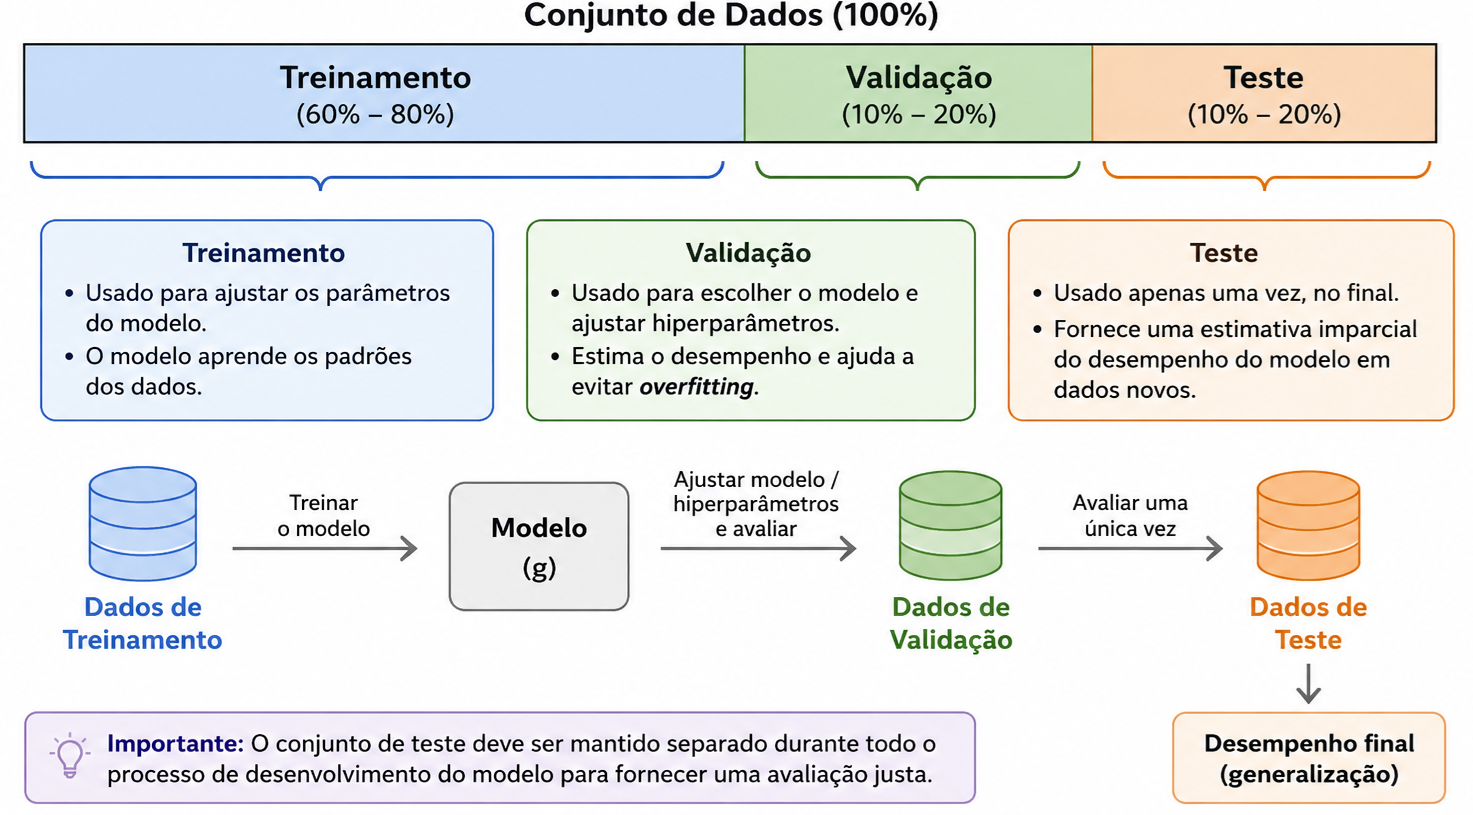
\includegraphics[keepaspectratio]{../../../images/classificacao/data_splitting.png}}
\end{center}
\end{frame}

\begin{frame}{Estimação do Risco e Seleção de Modelos}
\phantomsection\label{estimauxe7uxe3o-do-risco-e-seleuxe7uxe3o-de-modelos-1}
Assim,
\(\mathcal{D}=\mathcal{D}_{treino} \cup \mathcal{D}_{val} \cup \mathcal{D}_{teste}\).
Utilizamos o \textbf{conjunto de treinamento} para \textbf{estimar
\(g\)} e o \textbf{conjunto de validação} apenas para \textbf{estimar
\(R(g)\)} via

\[
\widehat{R}_{val}(g)
=
\frac{1}{n_{val}}
\sum_{(\mathbf{x}_i,Y_i)\in \mathcal{D}_{val}}
I(Y_i\neq g(\mathbf{x}_i)).
\]

isto é, avaliamos a \textbf{proporção de erros} no conjunto de
validação.
\end{frame}

\begin{frame}{Estimação do Risco e Seleção de Modelos}
\phantomsection\label{estimauxe7uxe3o-do-risco-e-seleuxe7uxe3o-de-modelos-2}
\begin{block}{Garantia teórica da validação}
\phantomsection\label{garantia-teuxf3rica-da-validauxe7uxe3o}
Sejam \(G = \{g_1,\cdots, g_N\}\) uma classe de classificadores
estimados com base em um conjunto de treinamento e,

\[
g^*
=
\arg\min_{g\in G}R(g)
\]

o melhor modelo verdadeiro estimado.

Seja \(\hat g=\arg\min_{g\in G}\hat R(g)\), o modelo escolhido via
validação.

\textbf{Resultado:} Com alta probabilidade, \(R(\hat g)\approx R(g^*)\).
\end{block}
\end{frame}

\begin{frame}{}
\phantomsection\label{section}
\end{frame}

\begin{frame}{}
\phantomsection\label{section-1}
\end{frame}

\begin{frame}{Balanço entre Viés e Variância}
\phantomsection\label{balanuxe7o-entre-viuxe9s-e-variuxe2ncia}
Assim como em regressão, em classificação também se enfrenta o paradigma
do \textbf{balanço entre viés e variância}.

\begin{block}{🎯 Ideia central}
\phantomsection\label{ideia-central}
Seja \(G=\{g_1,\dots,g_N\}\) uma classe de classificadores. Além disso,
sejam o \textbf{melhor risco} (risco do oráculo) que pode ser obtido
usando-se classificadores de \(G\) dado por

\[
R_{or}
=
\inf_{g\in G} R(g)
\]

e \(R_*\) o \textbf{risco do classificador de Bayes}.
\end{block}
\end{frame}

\begin{frame}
Para todo \(g \in G\),

\[
R(g)-R_* = T_1 + T_2
\]

onde:

\[
T_1 = R(g)-R_{or}
\]

é o \textbf{análogo da variância}.

✔ sensível aos dados de treino

✔ cresce com modelos muito flexíveis

✔ alto risco de overfitting
\end{frame}

\begin{frame}
Além disso,

\[
T_2 = R_{or}-R_*
\]

é o \textbf{análogo do viés ao quadrado}.

✔ erro devido à simplicidade do modelo

✔ alto em modelos muito rígidos

✔ causa underfitting
\end{frame}

\begin{frame}{Trade-off}
\phantomsection\label{trade-off}
\begin{center}

\includegraphics[width=0.9\linewidth,height=\textheight,keepaspectratio]{intro_files/figure-beamer/unnamed-chunk-1-1.png}
\end{center}
\end{frame}

\begin{frame}{Outras medidas de desempenho}
\phantomsection\label{outras-medidas-de-desempenho}
\begin{block}{Problema da acurácia}
\phantomsection\label{problema-da-acuruxe1cia}
A taxa de erro

\[
R(g)=P(Y\neq g(\mathbf{x}))
\]

nem sempre descreve adequadamente o desempenho de um classificador. Um
modelo pode apresentar:

\begin{itemize}
\tightlist
\item
  baixa taxa de erro;
\item
  alta acurácia;
\end{itemize}

e ainda assim possuir \textbf{desempenho ruim na classe minoritária}.
\end{block}
\end{frame}

\begin{frame}
\begin{block}{💡 Exemplo clássico}
\phantomsection\label{exemplo-cluxe1ssico}
Considere que uma base de dados com 1000 pacientes, sendo

\begin{itemize}
\tightlist
\item
  990 saudáveis
\item
  10 doentes
\end{itemize}

Um classificador trivial que \textbf{classifica} todos como
\textbf{saudáveis} apresenta:

\begin{itemize}
\tightlist
\item
  acurácia ≈ 99\%;
\item
  sensibilidade = 0
\end{itemize}

⚠️ O modelo falha completamente em \textbf{detectar pacientes doentes}.
\end{block}
\end{frame}

\begin{frame}
\begin{block}{Matriz de confusão}
\phantomsection\label{matriz-de-confusuxe3o}
\[
\begin{array}{c|cc}
 & \textbf{Valor verdadeiro} & \\
\textbf{Valor Predito} & Y=0 & Y=1 \\
\hline
Y=0 & \text{VN (verdadeiro negativo)} & \text{FN (falso negativo)} \\
Y=1 & \text{FP (falso positivo)} & \text{VP (verdadeiro positivo)}
\end{array}
\]
\end{block}
\end{frame}

\begin{frame}{Outras medidas de desempenho}
\phantomsection\label{outras-medidas-de-desempenho-1}
\begin{block}{Sensibilidade (Recall): Capacidade do modelo detectar
observações positivas}
\phantomsection\label{sensibilidade-recall-capacidade-do-modelo-detectar-observauxe7uxf5es-positivas}
\[
S=\frac{VP}{VP+FN}
\]
\end{block}

\begin{block}{Especificidade: Capacidade do modelo detectar observações
negativas}
\phantomsection\label{especificidade-capacidade-do-modelo-detectar-observauxe7uxf5es-negativas}
\[
E=\frac{VN}{VN+FP}
\]
\end{block}
\end{frame}

\begin{frame}{Outras medidas de desempenho}
\phantomsection\label{outras-medidas-de-desempenho-2}
\begin{block}{Precisão (Precision): Confiabilidade das predições
positivas}
\phantomsection\label{precisuxe3o-precision-confiabilidade-das-prediuxe7uxf5es-positivas}
\[
VPP=\frac{VP}{VP+FP}
\]
\end{block}

\begin{block}{Valor preditivo negativo: Confiabilidade das predições
negativas}
\phantomsection\label{valor-preditivo-negativo-confiabilidade-das-prediuxe7uxf5es-negativas}
\[
VPN=\frac{VN}{VN+FN}
\]
\end{block}
\end{frame}

\begin{frame}{Outras medidas de desempenho}
\phantomsection\label{outras-medidas-de-desempenho-3}
\begin{block}{Estatística \(F_1\)}
\phantomsection\label{estatuxedstica-f_1}
\[
F_1=
\frac{2}{\frac{1}{S}+\frac{1}{VPP}}
\]

Média harmônica entre:

\begin{itemize}
\tightlist
\item
  sensibilidade;
\item
  precisão.
\end{itemize}
\end{block}
\end{frame}

\begin{frame}{Interpretação probabilística}
\phantomsection\label{interpretauxe7uxe3o-probabiluxedstica}
As métricas derivadas da matriz de confusão estimam probabilidades
populacionais. Por exemplo:

\begin{block}{Sensibilidade}
\phantomsection\label{sensibilidade}
\[
S \approx P(\hat g(X)=1 \mid Y=1)
\]
\end{block}

\begin{block}{Especificidade}
\phantomsection\label{especificidade}
\[
E \approx P(\hat g(X)=0 \mid Y=0)
\]

{💡} Assim, é importante calcular os valores de VP, FN, VN e FP
utilizando uma \textbf{amostra de teste} ou \textbf{validação} para
evitar o \textbf{sobre-ajuste}.
\end{block}
\end{frame}




\end{document}
